\documentclass[11pt,a4paper,UTF8,fontset=macnew]{ctexrep}

\usepackage[margin=1in]{geometry}
\usepackage{graphicx}
\usepackage[dvipsnames,table]{xcolor}
\usepackage[colorlinks=true, linkcolor=NavyBlue, urlcolor=NavyBlue]{hyperref}
\usepackage{colortbl}
\usepackage{booktabs}
\usepackage{tabularx}
\usepackage{float}
\usepackage{enumitem}
\usepackage{longtable}
\usepackage{amsmath, amssymb}
\usepackage[most]{tcolorbox}
\usepackage{fancyhdr}

\setlist[itemize]{nosep, leftmargin=*, topsep=2pt, partopsep=0pt}
\setlist[enumerate]{nosep, leftmargin=*, topsep=2pt, partopsep=0pt}
\widowpenalty=10000
\clubpenalty=10000
\brokenpenalty=10000

\definecolor{acc}{HTML}{1F4E79}
\definecolor{warn}{HTML}{9C4221}
\definecolor{good}{HTML}{2F6042}
\definecolor{soft}{HTML}{F2F5F9}

\ctexset{
  chapter/format = \Huge\bfseries\color{acc},
  section/format = \large\bfseries\color{acc},
}

\pagestyle{fancy}
\fancyhf{}
\lhead{\small RPent 框架文档}
\rhead{\small\thepage}
\renewcommand{\headrulewidth}{0.4pt}

\newtcolorbox{evidence}[1][]{colback=soft, colframe=acc!70, fonttitle=\bfseries,
  boxrule=0.6pt, left=6pt, right=6pt, top=5pt, bottom=5pt, breakable, #1}
\newtcolorbox{caution}[1][]{colback=warn!5, colframe=warn!70, fonttitle=\bfseries,
  boxrule=0.6pt, left=6pt, right=6pt, top=5pt, bottom=5pt, breakable, #1}
\newtcolorbox{resolved}[1][]{colback=good!5, colframe=good!70, fonttitle=\bfseries,
  boxrule=0.6pt, left=6pt, right=6pt, top=5pt, bottom=5pt, breakable, #1}

% float placement: let tables share pages with text instead of stranding
\setcounter{topnumber}{2}
\setcounter{totalnumber}{3}
\renewcommand{\topfraction}{0.9}
\renewcommand{\bottomfraction}{0.7}
\renewcommand{\textfraction}{0.1}
\renewcommand{\floatpagefraction}{0.8}

\newcommand{\keyrule}[1]{\textbf{\textcolor{acc}{#1}}}

\title{\vspace{-2em}\textbf{RPent 智能体框架}\\[0.4em]
\large 从上游项目到一个会自己长大的系统：\\
架构、来龙去脉、实验，以及证据到底支持什么}
\author{RPent 框架项目}
\date{2026 年 8 月 12 日}

\begin{document}
\maketitle

\begin{abstract}
\noindent
这份文档记录的是一次重建。一个 LIBERO 操作基准任务，由一个纯文本的规划器
（\texttt{deepseek-v4-flash}）驱动，它从头到尾看不见任何图像；本文写的是围绕这个
固定的、便宜的模型所搭的那层框架——它通过什么工具动手、在什么边界内动手、留下什么
记录，以及它靠什么机制在一次次运行之间把知识攒下来。

叙述按照搭建顺序展开，因为每一层的存在都是为了让下一层可被测量。文末是四个实验臂、
一个受控消融，以及篇幅同样长的一节，专门写这个项目提出过、后来又不得不撤回的结论。
最后那部分不是谦虚。本文的核心主张是：一套框架值不值得搭，取决于它能不能说清自己值
多少；而一个连自己的错误都抓不出来的项目，并没有证明这一点。
\end{abstract}

\tableofcontents

% ==========================================================================
\chapter{总览}

\section{一页看懂这个系统}

三个 GPU 服务跑在 HTTP 边界后面：MuJoCo 环境、冻结的 Pi0.5 视觉-语言-动作策略，以及
负责分割的 SAM 3.0。它们前面是一个规划器——一个跑在回合循环里的语言模型——负责发出
工具调用、读取返回结果。\textbf{这个规划器在设计上就是瞎的}：启动时带
\texttt{-{}-no-images}，收不到任何像素；分割结果、世界坐标图和几何测量，就是它接触
场景的全部通道。

这个约束是刻意的，并且决定了后面的一切。瞎的规划器必须\emph{测量}而不是看，这意味着
它对世界的每一个判断都能追溯到某一次工具返回，也就意味着这次运行的记录可以被审计：
某个决定到底是挣来的，还是编出来的。项目的总原则由此而来——重数据留在磁盘上，进上下
文的只是引用。点云和图像永远不进提示词；工具读路径、算数字，规划器在结果之上做推理并
给出出处。

\section{两条定下大多数争论的规矩}

\keyrule{机制优于自觉。} 写在提示词里的规矩是自觉，卡在工具分发路径上的门是机制。凡是
两种做法都可行的地方，机制赢。最清楚的例子是沙箱（第 \ref{ch:sandbox} 章）：提示词里三条“不许读”的
禁令，变成了代码里的一份白名单；然后提示词干脆不再提那些文件——因为\textbf{为了禁止
而点名，本身就是在打广告}。

\keyrule{归因才是目的。} 这套基础设施存在的意义，是能说出某个组件到底值多少：值多少分、
值多少 token、什么时候反而有害。决策的评判标准，是它让归因变容易还是变难。正因如此，
中间件顺序是一个写死并声明出来的常量，每次运行都会把自己所处的边界指纹落盘，而第 \ref{ch:exp}
章的实验是围绕\textbf{单变量对照}组织的，而不是围绕一个好看的总分。

\section{改了些什么}

分叉点是上游 \texttt{RLinf/RPent} 的 \texttt{3c2516e3}。相对于它，这项工作大约是
六十个提交、120 个文件。

\begin{table}[htbp]
\centering\small
\begin{tabularx}{\textwidth}{@{}l X@{}}
\toprule
\textbf{层} & \textbf{改动} \\
\midrule
工具层 & 一个 1{,}930 行的模块拆成 15 个文件的包；手写 schema 字典换成框架原生工具；五跳分发变两跳 \\
描述 & 模型能读到的关于工具的每一个字，收进唯一一份结构化、带 lint 的来源 \\
提示词 & 先删掉逐格答案；再让提示词随沙箱的\emph{能力}变化，而不是随它的名字变化 \\
沙箱 & 常开、失败即关闭的文件边界；配置即数据；先验下载改成按需、落到暂存区 \\
证据层 & 每一次工具调用都记录，包括只读调用；只追加的实体数据总线；只凭磁盘产物重建回放 \\
提升门 & 五项检查的晋升流水线，带人工中断，是记忆库的唯一写入者 \\
制度 & 练习种子与考试种子在代码里分开；实验回合；驻场多次尝试调试会话 \\
感知 & 一个可查询的视觉仪器，以工具的形式加入，而不是换模型 \\
\bottomrule
\end{tabularx}
\end{table}

% ==========================================================================
\chapter{起点}

上游那套框架是能跑的，其中两点被判定为“好到不该重写”：感知与动作是分开的；特权信息是
在代码里扣住的，而不是在提示词里客气地请求不要看。项目负责人给的指示是：\textbf{包起
来、扩出去，不要重构}。

真正需要改的是另一类东西。\texttt{robots/libero/tools.py} 有 1{,}930 行，把运动原语、
策略桥接、分割、几何、状态落盘和手写的工具 schema 字典塞在同一个命名空间里。一次调用
要经过五跳才能走到实现：注册表查找、spec 字典、名字字符串、属性查找、偏函数、handler。
单看每一跳都没错。问题在于，五跳意味着有五个地方可以忘记某个横切关注点，而本文里的每
一个机制都是横切关注点。

代码旁边才是测量真正的障碍。提示词里带着 t0 到 t9 的逐任务配方，连坐标都在。一份 187
个数字常量的标定手册每次运行都注入。还有一个装着逐格解法的资源目录，\emph{每次运行}
都从模型仓库重新下载并覆盖——也就是说，本地把答案删了并不算数。

\begin{caution}[title={这让测量变得不可能}]
事后从日志里数出来：那个时期的 155 次运行中，\textbf{104 次读了被打分那一格的答案
文件}，89 次读了标定表。那段时间产生的任何数字都不是在测量一套框架，而是在测量一次
查表。
\end{caution}

% ==========================================================================
\chapter{工具层}

\section{从一个模块到一个包}

模块按工具种类拆成十五个文件：几何、状态、感知、运动、策略桥接、schema、描述、上下文、
数据总线、产物布局，外加一个不依赖任何东西的小目录表。总行数从 1{,}930 涨到 4{,}481
——这个算术需要老实交代：\textbf{这不是纯粹的拆分}。十五个模块里有六个，是此前根本不
以代码形式存在的关注点。

工具现在是框架原生工具：一个装饰器、一份带类型的参数 schema、一个携带运行时上下文的
参数。一个完整的工具短到可以整个读完。

\begin{evidence}[title={一个工具，从头到尾}]
\ttfamily\footnotesize
@tool(args\_schema=Pi0PickInput, description=tool\_docs.render\_description("pi0\_pick"))\\
def pi0\_pick(prompt, runtime, max\_chunks=24, lift\_thresh=0.05, ...):\\
\hspace*{2em}"""面向模型的文字由 tool\_docs 渲染——要改去那里改。"""\\
\hspace*{2em}ctx = \_context(runtime)\\
\hspace*{2em}return ctx.advance("pi0\_pick", \{...\}, ctx.primitives.pi0\_pick)
\end{evidence}

\noindent
分发是两跳：工具函数、\texttt{ctx.advance}、原语。没有名字字符串查找，没有偏函数，
没有分发表。

\section{为什么这不是表面功夫}

\texttt{ctx.advance} 成了\textbf{所有推进环境的调用都必须经过的唯一接缝}，而且它独占
每次动作的全部记账：计时、取消、动作视频切片、步数递增、数据总线里的新鲜度降级、状态
落盘，以及把新状态渲染回规划器。没有任何一个工具重新实现其中任何一项，也没有任何一个
工具\emph{有机会忘记}。

正是这条唯一接缝，让后面的证据层、尝试轮转和沙箱写保护得以成为\emph{机制}，而不是
\emph{约定}。它也是证据层发现的一个缺陷的修复处：已经结束的回合不能再走一步，现在这里
返回一条解释性的错误而不是崩溃——因为实验回合经常在意外解开之后继续探查，一次迟到的
调用不该让整轮运行丢掉自己的笔记。

“哪些调用会改变世界”这套词汇，住在一个 32 行、不 import 任何东西的模块里，而且\textbf{不
可能漂移}：如果工具模块自己的推进工具清单和这份目录表对不上，import 时就抛异常。

\section{三个值得写下来的决定}

\keyrule{永远不要给工具模块加延迟注解求值。} 框架靠把注解解析成真实类型来识别运行时参数。
在延迟求值下它看到的是一个字符串，注入静默失败，于是每一次工具调用都会死在\emph{分发
时，而不是 import 时}。仓库里其它每个模块都有那行 import，所以这恰恰是一次“顺手整理”
的提交最容易“修好”的东西。

\keyrule{schema 用类型化模型，而且这是一次翻案。} 第一版适配器原封不动地把已有的 schema
字典透传过去，好让面向模型的表面在迁移前后可以被\emph{证明}是同一份。负责人推翻了它：
一份定义应该同时给出校验、schema 和类型。代价被明确接受——渲染出来的 schema 形状变了，
所以那份相等性证明作废。

\keyrule{两个命名空间，两边的名字都对。} 十四个工具里有九个包着 mixin 方法，而装饰器不
能装饰方法。合并命名空间就得把每个物理函数改名，好让工具占用那个好名字。有五个工具名
与它们的 handler 撞名，这也是模块把兄弟模块当命名空间 import、而不是 import 其成员的
原因。

\section{与上游的趋同}

上游后来独立地朝同一个方向走了一段：一个较新的提交引入了按运行持有步骤轨迹与产物存储
的状态对象，以及一个把 handler 标为只读的装饰器，好让其余 handler 默认抓取一次观测。
这与这里得出的“推进/只读”划分是同一个直觉。差别在落点，而那正是第 \ref{ch:evidence} 章的主题：\textbf{他
们把状态采集集中化了，我们把证据记录集中化了}——包括那些什么都不改变的调用。

% ==========================================================================
\chapter{模型能读到的一切，只有一个来源}

关于一个工具，模型被告知的一切都住在两个文件里：一份结构化的描述条目，以及参数 schema
——后者的字段描述同样属于面向模型的表面。Python 的 docstring 是给开发者看的注记，并且
它自己就这么写着。

描述模板有六个字段，字段之间的边界才是有意思的部分。前置条件里不许复述参数，因为参数
只在 schema 里记录、别处一概不记。选择指引里不许编码工作流位置，因为流程顺序归系统提示
词管。用法说明里不许写跨工具的多步流程——用模板自己的话说，“配方就是这样爬回工具描述
里的”。定量的警示必须有测量背书。

内容是从迁移前的 docstring \textbf{逐字}搬过来的：句子被搬进字段，而不是被重写。理由是
面向模型的表面是一个实验变量，所以措辞的改动必须是刻意的、被测量的，不能夹带在一次重构
里偷偷进来。

之所以要这么讲究，还是为了归因。那个表面必须是一个\emph{表面}——可哈希、可 diff、可
lint——而不是散落各处的 docstring。一个只依赖标准库的测试把它维持成一个整体，共六项检查：
import 时校验、手工维护的名册（这样改名会显眼地报错）、已记录工具与真实工具的对称比对、
悬空引用 lint，以及渲染源与两套分发底座之间的逐字节一致。第六项是承重的那一项：

\begin{evidence}[title={先验泄漏 lint，跑在模型真正看到的渲染字节上}]
\ttfamily\footnotesize
FORBIDDEN\_PATTERNS = [r"resources/", r"results\_\textbackslash w*", r"env\_calibration",\\
\hspace*{6em} r"guides/", r"past recipe", r"memory file", r"memory librar", r"MEMORY\textbackslash .md"]
\end{evidence}

\noindent
有一个模式会贯穿本文余下的部分：\textbf{随运行时开关变化的能力，各有各的描述条目，绝不
用一份静态的超集描述}。在 \texttt{-{}-no-images} 下，读图工具被换成一个如实说明自己
做不到的变体，而不是继续承诺它给不了的东西。

% ==========================================================================
\chapter{提示词，以及让它变诚实的那个沙箱}
\label{ch:sandbox}

\section{清洗：准入规则}

提示词掉了 42\% 的字节——源文件从 33{,}463 降到 19{,}544——而删掉的是什么，比数字更有
意思。被删的有：逐任务配方块及其坐标；一节与工具 schema 默认值重复的超参；一个形如
\texttt{eef\_y = plate\_y + 0.045} 的常量（后来测量把它推翻了：同一次运行内，同一个
偏移量在 1.0 到 4.1 厘米之间浮动）；那条让智能体去读 seed-0 参考答案的工作流步骤——它
本身就是泄漏通道；以及那份 187 个常量的标定表。

筛选标准\emph{不是}“含不含数字”。那个标准两头都错——抽屉的区域边界是数字、是不变量、
而且感知上无法恢复，那就是知识；“深色那瓶是沙拉酱”一个数字都没有，却是纯答案。真正的
规则是二维的。

\begin{table}[htbp]
\centering\small
\begin{tabularx}{0.94\textwidth}{@{}l X X@{}}
\toprule
 & \textbf{随实例变化} & \textbf{不变} \\
\midrule
\textbf{工具能测出来} & 永远不进提示词——去测 & 最多写成一条检查，绝不写成一个值 \\
\textbf{工具恢复不了} & 这就是作弊：某一格的答案 & \textbf{唯一配得上这些 token 的一类} \\
\bottomrule
\end{tabularx}
\end{table}

\noindent
活下来的有：坐标系约定、夹爪语义、哪个原语会穿过运动学奇异点、腕部相机的模态弱点，以及
“运动失速”的判定。

\section{分级：把广告也删掉}

清洗删的是答案，分级删的是\emph{广告}。提示词现在随沙箱\emph{实际允许什么}变化，而不
随配置的名字变化：只有当记忆库的根目录确实可读时，库相关的指令才存在——而这是从活的
策略对象上探测出来的，不是从命令行读的。一个自定义配置只要暴露了库，就自动拿到库的
指令，不管它叫什么名字。

负责人坚持的那个推论，是最让人意外的一条。\keyrule{每一条口头的文件禁令都被删掉了，所有
变体都是。} 那些“不许读解法”“不许读标定表”的禁令块，是拿自觉去顶一个缺失的机制。沙箱
一旦存在，它们就成了纯粹的广告：点名一个被封的文件，等于告诉模型它存在、以及里面有什么。
现在无先验的提示词读起来就像那些文件从来没存在过，而一个 44 条断言的 lint 强制这一点
——一份禁止字符串词表，在\emph{任何}变体里都不许出现；外加反方向：考试变体里不许出现
它并不携带的驻场工具的名字。

完整的能力阶梯——无库、有库、库加任务小本子、再加驻场制度——渲染后跨度是 20{,}551 到
21{,}959 个字符。占提示词不到 7\%，这正是它能作为一个干净归因轴的原因。

\section{沙箱}

\keyrule{常开。} 没有关闭开关。“不带边界地调试”是一个具名配置，其运行会自我声明“什么都
没测到”。在策略被初始化之前，每一项检查都\textbf{失败即关闭}，所以泄漏不可能因为忘了
加一个 flag 而发生。

\keyrule{配置即数据。} 五个简短的 YAML 文件引用占位符，按运行解析。代码从不对配置名做
特判，未知键直接报错。

\keyrule{配置声明意图，代码守住不变量。} 写保护路径集合\emph{不在}允许的键里——它根本
无法在配置中声明。它是从产物布局表推导出来的，所以新增一类产物是\textbf{按构造}就受
保护，而不是靠记得。\emph{一个能改写自己证据日志的智能体，会让所有归因主张失效}，所以
这条边界不是配置。每一个出厂配置，包括最宽松的那个，都只允许在本次运行目录内写入。

\keyrule{同步改成按需且落暂存区。} 那个原本每次运行都覆盖资源目录的下载，现在只在当前
配置引用了暂存根时才发生，目标是暂存路径而不是活目录，已有副本会复用，而且——刻意地
——没有异常处理：部分同步会抛出，而不是继续跑。一个跑在悄悄残缺的载荷上的对照臂，什么
都测不到。

\section{删掉旧记忆}

沙箱只是一半。从模型仓库来的那个库里，仍然躺着那个被推翻的常量。\textbf{清洗了提示词
并没有清洗库}。解决办法不是去改旧库，而是不再注入它，并在门的管控下\textbf{从零重建
一个}。现在的库有 21 条通用条目和一批不断增加的任务级条目，没有一条早于这项工作，而且
每一条都带着它被挖出来时所依据的运行引用。

\begin{table}[htbp]
\centering\small
\begin{tabular}{@{}l c c c@{}}
\toprule
\textbf{时期} & \textbf{运行数} & \textbf{读了答案文件} & \textbf{读了标定表} \\
\midrule
重构前 & 155 & \textbf{104（67\%）} & 89 \\
本框架，沙箱之前 & 11 & 1 & 11 \\
本框架，沙箱开启 & 136 & \textbf{0} & \textbf{0} \\
\bottomrule
\end{tabular}
\caption{沙箱的验收测试，从运行日志中统计。}
\end{table}

% ==========================================================================
\chapter{证据层}
\label{ch:evidence}

\section{把“什么都没改变”的调用也记下来}

只有当某个原语推进了环境，步骤轨迹才会多一条记录。在被检查的一次运行里，发生了 27 次
工具调用，而轨迹里只有 6 条。关于感知和文件读取的一切——\textbf{包括智能体有没有去读
答案}——完全不可见。

现在有一个中间件在工具分发的包装层里为每次调用写一行，那是唯一能统一看到所有调用的
接缝。普适性是结构性的，而不是靠政策：钩子包住的是分发器，所以没有名字过滤，也没有
“这个工具推不推进环境”的分支。崩掉的工具会被记录然后重新抛出。步数在 handler 两侧各采
一次，于是\emph{“这次调用有没有推进环境”是从日志里算出来的，而不是在日志里声明的}，
而只读调用被钉在它所观测的那个状态上。

写入器永远不抛异常——少一行日志，比毁掉一整个回合损失小；追加时加锁，因为同一回合的
调用是并发的；除标准库外什么都不 import，这样诊断脚本不装智能体框架也能读一次运行。

中间件顺序是一个声明出来的常量，理由就写在旁边：\emph{顺序不同就是方法不同，所以要记录
下来，而不是让它隐含存在}。九条里有四条尚未实现，且是刻意具名的——因为把一个已知的
缺口写下来，比将来重新发现它便宜。

\section{实体数据总线}

具名实体的读数只追加、从不改写。一个可变的“当前位置”会摧毁 provenance，而 provenance
的存在，正是为了让一次运动能引用它据以规划的那次读数。\textbf{刻意不提供求平均}：容器
近壁的两次读数，偏差可能相互抵消；但一次抓到物体主体、一次抓到瓶盖的两个读数，平均出来
的点两者都不是。

新鲜度由框架计算、由规划器解释。四种判定依据到末端执行器路径的实测距离给出，而 docstring
把近似说明白而不是藏起来——只知道动作前后的位姿，所以一个下探再抬回原处的策略调用对这
个检验是不可见的。\textbf{判定是扰动的下界}，“未验证”意思是\emph{不知道有没有被扰动}，
绝不是\emph{已知没被碰过}。

冲突只报告、从不裁决。两个不同名字的实体落在三厘米内会触发碰撞告警——这个阈值来自数据：
真实桌面物体实测相距 6 到 20 厘米，而同一物体的重复读数彼此吻合到毫米级。检测器在同一段
注释里说明了自己的能力边界：它抓的是碰撞，不是\emph{对调}；两个物体在两个位置上、标签
互换，几何上是自洽的。

\section{回放是一次完整性测试}

回放\textbf{只凭磁盘产物}把一次跑完的运行重建成逐回合时间线，并把自己的不完整以“记录
缺口”为标题渲染出来。这个约束正是它的价值：出现缺口意味着日志缺东西，补救办法是\emph{多
记}，而不是改进渲染器。

调用日志与转录之间的连接是按位置并带名字校验的，一旦对不上就降级为警告，而不是把推理
安到错的调用上。渲染器只读；唯一被允许的推导，是把记录下来的世界坐标投影到记录下来的
相机图像上；投影误差超过五厘米的点会画成警告线，而不是一个自信的圆点。

\section{这一层抓到了什么}

\begin{itemize}
\item 策略的成功标志\emph{恰恰在预置位做得好的时候}是假的，因为它的判据要求下探十厘米。
      它惩罚的正是提示词教它做的事。
\item 夹爪宽度检测不出抓握：某次运行连续五步宽度相同，而点云在前三步里在末端执行器下方
      什么都没找到。
\item 一个几何工具把桌面报成了被抓物体——六次运行的 25 个闭爪步里，有十二个读的是一个
      平面。
\item 掩膜边缘溢出让每一次尺寸测量都偏大，最严重的一例是六倍。
\item 一个比较工具无法区分成功与失败：四次释放中，解开的运行与从未终止的运行签名无法
      区分，因为搁在边沿上的物体和坐进去的物体读数一样。这条以否定结果的形式报告，并
      写进了该工具自己的契约。
\end{itemize}

% ==========================================================================
\chapter{提升门}

\section{分层消化}

知识要进库得过五道：对单次运行的观察（对现有库是盲的）、跨扫描的综合（看得到全部）、
机械审查、人工中断、以及执行。观察者对库是盲的，这正是“某条主张的支持度可以从\emph{独立
发现}中计数”的前提，而不是从“和已经写下来的东西一致”中计数。

\keyrule{反传闻的铁律。} 提案证据必须落到引用 token 上，并直接解析进逐调用日志，\textbf{绝
不落到观察文件上}——观察文件本身就是模型输出。一套语法覆盖工具调用、环境步和产物；解析
器把 token 解引用成真实记录，返回工具名、参数、状态和结果，于是审查者读到的是\emph{记录
说了什么}，而不是\emph{提案声称记录说了什么}。没有引用的提案在被读之前就被拒。

\section{五项检查}

它们是同一趟检查里五个带标签的段落，各自给自己的发现打标记。

\begin{enumerate}
\item \textbf{契约}——每条引用都必须能解引用；改动已有条目会自动触发一个 flag。这里一旦
      出现拒绝就短路，因为一个无法评估的提案往下只会制造噪声。
\item \textbf{数字}——正文里的每个数字都必须在某条被引用的记录里出现（允许舍入误差），
      否则：\emph{要么引用那次测量，要么把数字删掉}。
\item \textbf{逐格答案}——分层处理。任务层可以点名某一格的物体，因为那正是它的用途；但
      绝对坐标会被 flag，因为它们随种子一起死。在通用层，任何与被引用运行里真实物体名
      匹配的 token 都被标为“这是答案，不是知识”——而那份词表是\emph{从运行里测出来的}，
      不是硬编码的。
\item \textbf{作用域}——一条自称跨环境却点了环境名字的主张，多半应该是环境级。
\item \textbf{去重}——与库内条目、以及与同批兄弟提案的相似度。
\end{enumerate}

\noindent
外加第六条没有编号的规矩，一句话概括了全部认识论：\emph{支持度是数出来的，不是声称出来
的。}

\section{中断，以及唯一的写入者}

审查产出一份判决文件，里面有两个分开的字段：机器的建议，作为不可变记录保留；以及\emph{人
的那一行}，仅仅用建议预填。执行阶段做严格相等比对——任何不是字面 “admit” 的都连同理由
一起归档——并在写入前重新校验契约。

“执行阶段是库的唯一写入者”同样不是一个约定：每一个沙箱配置都只允许在运行目录内写入，
所以智能体在物理上就写不到库里。它的提案落到一个子目录里，等门来裁决。

四个动词编码了一条不对称的证据门槛——\textbf{进门宽，续任严，靠反驳出局}。支持度由被引用
的不同运行数推导，而不是取声明字段；provenance 只追加、从不覆盖；而“驱逐”会先带日期戳
\emph{归档}再移除，因为一次驱逐是一个否定结果，不是一次删除。

\section{世代协议，以及它诚实的结果}

清空、扫描、挖掘、审查、执行、再来一轮。总共跑了五代，单次成绩读起来是
$4 \to 5 \to 7 \to 6 \to 5$：一条增长曲线。

\begin{caution}[title={曲线死了，接替它的数字也死了}]
在重复实验下，这条曲线消失了。接替它的那个数字——记忆库值 $+0.7$ 格——也死了：在当前
代码上重跑一次无库扫描，得了 6 分，于是暴露出早先那个低分是一次请求完整性崩溃的牺牲品，
而那个 bug 早已修好。\textbf{没有任何一层库能带来可测量的全套提升}：无库、已晋升记忆、
以及盲态任务小本子，在 6.0 上无法区分。两个主张都已撤回。
\end{caution}

\noindent
这套协议\emph{确实}证明了的是：审查过程本身在可测量地变好——五轮下来，需要人工修补的
次数依次是 1、4、1、1，最后是 0。而账本给出了别的仪器给不出的发现：第二代起“翻库”变得
有选择性，救回了两格；而同样的选择性让一条反螺旋条目成了孤儿，它所针对的那一格正在螺旋
时，它却没人读。

% ==========================================================================
\chapter{制度：练习、考试、驻场}

\section{种子划分}

51 及以上是练习种子，更小的是计分种子。练习种子上学到的知识可以进库；计分种子只考一次、
单次尝试，永远不从它身上学。这条在参数解析处强制执行，而不是写在文档里，而且拒绝时会
把理由说出来：在计分种子上做多次尝试会污染它。

实验回合把任务简报换成“试验与结论”简报：针对一个开放问题做受控试验，每次只改一个变量，
并用能在重新随机化的场景中存活的相对量写下结论。任务小本子给库加了一个按格划分的层，
挖掘和过门的方式与通用层完全一致。

\section{驻场调试会话}

负责人要的是某篇已发表的智能体系统那种调试方式。第一版做成了回合之间的循环，负责人两次
反驳，而且都对：那是“反思-重试”，而参考系统是在\emph{任务之内}调试。重读之后，真正要紧
的区别是：参考系统的调试器是一个\textbf{驻场会话}——每个任务一个长上下文会话，写、执行、
读轨迹、打补丁、再执行，全都在同一个记得住每一次先前尝试的连续上下文里。回合之间的循环，
每轮召唤的是一个失忆的更新器。

负责人的洞察让它变得很便宜：\textbf{回合循环本身已经是一个活的会话}。挡住驻场的是三堵
自设的墙，每一堵都换成了一个机制。

\begin{table}[htbp]
\centering\small
\begin{tabularx}{\textwidth}{@{}X X@{}}
\toprule
\textbf{墙} & \textbf{机制} \\
\midrule
回合边界等于会话边界 & 一个按能力开放的重置工具 \\
单次尝试制度（对考试是对的） & 把尝试轮转进归档目录 \\
上下文预算 & 逐尝试折叠，\emph{并配一个检索通道} \\
\bottomrule
\end{tabularx}
\end{table}

\keyrule{工具是否存在，就是制度边界。} 重置工具只在驻场开关下出厂，而启动器在计分种子上
会拒绝该开关。\textbf{一次考试运行不可能被说服去重置，因为那个工具根本不在它的工具面
上}。提示词也同步分级：驻场变体\emph{替换}掉单次尝试那一段，而不是叠加——因为一边禁止
重置、一边又把重置工具发出去的提示词，是在宣告一条假的边界。

\keyrule{只有配上检索，折叠才成立。} 把工具消息折叠成摘要会丢信息——除非每条摘要是一个
\emph{索引项}而不是一段总结。每条被折叠的结果变成一行，带着它的引用键；另有一个专门的
工具把这个键解析回完整的归档记录。直接去读归档日志的方案被考虑并否决了：它从头开始读且
有字符上限，要够到第 37 次调用就得把 1 到 36 次重新灌回上下文，折叠也就白做了。

还有两条性质是刻意的。折叠是\emph{按请求生成的视图}，不是状态改写，所以磁盘记录保持完整、
回放看得到一切。而它是这个系统里第一次\emph{正当的}上下文压缩：归档是不可变的，因此被
折叠的前缀逐字节稳定，供应商的自动前缀缓存能保持命中——不像在消息中段做摘要，那会让缓存
从改写点开始整段失效。

轮转本身承载证据分量。归档目录在被创建的那一刻就注册为写保护，因为\textbf{一次失败尝试
的证据，必须活得比制造它的那个会话更久}。尝试清单里记录模型自己的诊断，schema 要求该字段
至少二十个字符：\emph{没有说明改了什么就重置，那是重跑，不是调试。}

% ==========================================================================
\chapter{视觉仪器}

t5 暴露的墙既不是知识也不是策略。那个用来区分的属性——两个相似容器里哪个是目标——\textbf{没
有任何测量通道}。几何分不开它们，分割把六个名词塌缩到同一个位置上。这从内部看是什么样子
值得引用，因为那正是“可测量的选项用完了”对一个推理模型的作用：

\begin{evidence}[title={盲态会话，第 16 回合，然后是第 18--19 回合}]
\small\emph{“对 A 的腕部探测全都在噪声范围内（tomato 0.551、bbq 0.574、red 0.637、
brown 0.602）——语言分不开这两个酱料瓶。”}

\medskip\ttfamily\footnotesize
turn 17\quad out=35{,}814\qquad turn 18\quad out=44{,}006\qquad turn 19\quad out=52{,}198
\end{evidence}

\noindent
第 18 和第 19 回合没有输出任何文字、也没有任何工具调用，各自消耗了\textbf{恰好 8{,}192}
个输出 token——整个生成预算，全烧在隐藏的推理通道里。运行死在第 19 回合，而上限是 150。
它不是在任务上失败；它是想靠“想”来解决一个感知问题。

因此视觉是以\textbf{工具}的形式进来的，不是换规划器、也不是注入——这种“拉取式”的形态，
正符合“规划器负责推理、工具负责测量”这条规矩。设计承诺：

\keyrule{逐字管道。} 回复原样透传：不摘要、不过滤、不抽取答案、不截断。

\keyrule{发出去的原文会被记录。} 中间人做了什么，仅凭运行记录就可审计。

\keyrule{读图者拿不到任何任务上下文。} 一行固定的系统消息，加上规划器的问题。读图者回答
的是像素；它不知道任务是什么，所以它无法把一个任务决策夹带着绕过规划器。

\keyrule{答案是意见，不是测量。} 文档里写明要用几何去交叉验证。

\keyrule{按臂门控并纳入沙箱。} 只有通道被装配时工具才出厂——\emph{盲臂不发一个它无法兑现
的工具}——而且它同样受沙箱管辖，否则它就是一个披着问号的字节外泄通道。

论点就是这个解耦本身：推理跑在一个便宜模型上，感知跑在另一个上，谁也不被要求去当对方。
结构性的理由是归因——一个单体多模态模型让感知通道不可测量，因为\textbf{没有接缝}。这里
接缝只有一个 flag 宽，而每一次跨越都是一条带图像路径的日志记录。

在同一个会话里，这个通道既救过场也误导过。一次像素回答反投影到桌面高度，重新抓取成功了；
另一次反投影到牛奶盒的高度，而当同一视角被重新裁剪再问一次时，读图者回答说中间那个物体
\emph{就是}牛奶盒、看不到目标。正是这一对，让最终被采纳的规则是一条\textbf{高度合理性
检查}，而不是一条禁令。

% ==========================================================================
\chapter{实验}
\label{ch:exp}

\section{一次“解开”怎么算}
\label{sec:counting}

事实基准是环境自己的终止标志，以步骤轨迹里记录的为准。三种较弱的信号因为可测的理由被
拒绝。\textbf{不用智能体的审计文件}：它只在智能体调用 finish 时才写，于是一次“解开之后
预算耗尽”的运行会被算成失败——这在整个归档里已经吃掉了五次真实的解开。\textbf{不用策略
的成功标志}：它在好的抓握上是假、在空抓上是真。\textbf{也不能跨代码库沿用同一个键}：
上游删掉了本项目使用的那个字段，改写成另一个名字、装在另一种容器形状里，所以按一种形状
写的计数器在另一种上会数出零，而且看起来像个结果。

\keyrule{被打断的运行是排除，不是计分。} 半路被杀掉的运行是一次缺失的测量，既不算失败也
不算解开。排除需要\emph{同时}满足：日志里没有自然退出标记，\emph{并且}时间戳与一次有据
可查的中止吻合。把这个检验用到整个归档上，找出四个候选：三个被排除，一个被保留——因为它
已经记下了自己的退出原因、然后死在清理阶段，这让它的测量是完整的。\textbf{只用一个条件
的规则会删掉一次真实的失败，并把某个臂的成绩抬高。}

\section{四个臂}

\begin{table}[htbp]
\centering\small
\begin{tabularx}{\textwidth}{@{}l l c X@{}}
\toprule
\textbf{臂} & \textbf{成绩} & \textbf{n} & \textbf{构成} \\
\midrule
上游，先验开启 & \textbf{8/10} & 1 & 上游提示词与规划器；\textbf{10/10 次运行共 112 次答案文件读取} \\
净室，无库 & \textbf{6.0}（6、6、6） & 3 & 沙箱开启、空库、0 次先验读取 \\
净室 + 库 & \textbf{6.0}（7、5、6） & 3 & 加上已晋升记忆与任务小本子 \\
\rowcolor{soft} 完整设计 & \textbf{8.0\,$\pm$\,1.0}（9、7、8） & 3 & 再加视觉仪器 \\
\rowcolor{soft} 完整设计，修好的库 & \textbf{8.67\,$\pm$\,0.58}（9、9、8） & 3 & 5f 已关闭、t9 驻场成果已入库 \\
\bottomrule
\end{tabularx}
\end{table}

\noindent
上游那个分数是\textbf{买来的}，而且发票在某一格里看得一清二楚。t5——这个让本项目付出了
一次驻场会话、一件仪器和三条经裁决的库条目的格子——上游在\textbf{环境第 2 步}就解开了：
先把那一格的答案文件读了三遍，然后两次一模一样的策略调用，\textbf{全程没有任何感知}。
这不是批评：答案就在磁盘上时，这是理性选择，而先验本来就是那套设计的一部分。它只是说明，
这个数字不能被读成对\emph{一套框架}的测量。

\section{受控消融}

盲态库臂，对比同一个臂装上仪器：同样的沙箱、同样的库、同样的模型、同样的预算、同样的
格子，各三趟。\textbf{仪器开关是唯一的变量}，本项目里没有第二个这么干净的对照。

\begin{table}[htbp]
\centering\small
\begin{tabular}{@{}l c c c l@{}}
\toprule
\textbf{格} & \textbf{盲态} & \textbf{带仪器} & \textbf{$\Delta$} & \textbf{读法} \\
\midrule
t0 & 0/3 & \textbf{3/3} & \textbf{+3} & 未预测；结果全靠它 \\
t1 & 3/3 & 2/3 & $-1$ & 噪声 \\
t2 & 3/3 & 3/3 & 0 & 已饱和 \\
t3 & 2/3 & 3/3 & $+1$ & 噪声 \\
t4 & 2/3 & 3/3 & $+1$ & 噪声 \\
t5 & 0/3 & 1/3 & $+1$ & 设计针对的目标——只动了一点 \\
t6 & 2/3 & 2/3 & 0 & 知识受限；预测为对视觉无感 \\
t7 & 3/3 & 3/3 & 0 & 已饱和 \\
t8 & 0/3 & \textbf{3/3} & \textbf{+3} & 未预测；结果全靠它 \\
t9 & 3/3 & \textbf{1/3} & \textbf{$-2$} & 回退，见 §\ref{sec:losses} \\
\midrule
\textbf{全套} & \textbf{6.0} & \textbf{8.0} & \textbf{+2.0} & \\
\bottomrule
\end{tabular}
\end{table}

\noindent
\textbf{全套的增益就是两格。} 在记录里，这六次运行中仪器都被用在早期、用于物体身份区分
——正是它被设计的用途——但其中有些回答\emph{是错的}，而且不存在配对的反事实。\textbf{对
这两格不做任何因果主张。}

\keyrule{装上不等于用上。} 三十次仪器臂运行里有三次带着开关却从未调用工具。它们实质上是
坐在仪器列里的盲态运行，这让 $+2.0$ 略微\emph{低估}了“使用”仪器的价值，同时略微高估了
“装上”仪器的价值。

\section{数字出现之前就已归档的预测}

\begin{table}[htbp]
\centering\small
\begin{tabularx}{\textwidth}{@{}X l@{}}
\toprule
\textbf{预测} & \textbf{结果} \\
\midrule
t5 应该动；它是设计针对的目标 & \textbf{部分错误}——0/3 到 1/3，且不是因为预测的那个原因 \\
t6 不变；它的墙是知识 & \textbf{正确} \\
t1、t2、t7、t9 已饱和、不变 & \textbf{t9 错了} \\
t3、t4 由噪声主导 & 正确 \\
t0、t8：明确拒绝预测 & 各自 0/3 到 \textbf{3/3}——增益全在这里 \\
\bottomrule
\end{tabularx}
\end{table}

\noindent
这个机制模型\textbf{对“价值会出现在哪里”判断错了}。它是为某一格造的，并预测在别处无关；
结果它几乎没动那一格，却扛起了另外两格。对那两个长期失败的格子拒绝预测是对的，而它们
之所以不可预测，是因为从来没有人诊断过它们为什么失败。

有一条归档下来的承诺必须用在它自己的作者身上：预注册里写明，“目标格没动、全套却大涨”是
唯一一个应当一眼就怀疑的结果——而这恰恰发生了。这条规则没有触发，因为位移集中在两个长期
为零的格子上、各 $+3$，这不是三个样本的噪声造得出来的——但它被记录下来，而不是悄悄丢掉。

\section{损失从哪里来}
\label{sec:losses}

仪器臂六次失败中有四次，\textbf{智能体自认为已经成功}。这既不是感知失败也不是策略失败，
而是\textbf{停止与自我报告的失败}，其成因是 §\ref{sec:5f} 的主题。

t9 的回退是其中一部分。预注册的解释——回合被仪器调用烧掉了——被记录\textbf{反驳}：两次
失败中有一次\emph{零次}调用仪器，而且两次都恰好用了 46 次工具调用。两次都抓对了物体、
抓握真实，然后提前停下了。

\section{第七代：这次修复，以及它赔掉的那一格}

关掉“停止许可”那个缺陷、并把 t9 驻场会话的成果挖进库之后，得到一个修好的库。又跑三趟：
\textbf{9、9、8——均值 8.67\,$\pm$\,0.58}。两个针对性的格子都动了，而 t5 在两批独立测量
中已经是修复后 \textbf{6/6}。

\begin{table}[htbp]
\centering\small
\begin{tabular}{@{}l c c c@{}}
\toprule
\textbf{格} & \textbf{盲态} & \textbf{带仪器} & \textbf{仪器 + 修好的库} \\
\midrule
t5 & 0/3 & 1/3 & \textbf{3/3} \\
t9 & 3/3 & 1/3 & \textbf{3/3} \\
\textbf{t1} & 3/3 & 2/3 & \textbf{0/3} \\
\bottomrule
\end{tabular}
\end{table}

\noindent
\textbf{而 t1 掉到了 0/3。}第一反应的怀疑是：条目修订把它弄坏了——\textbf{拆东墙补西墙}。
并没有。而且定案的论证是结构性的，不是统计性的：

\begin{caution}[title={为什么“靠许可拿到的解开”根本不可能被拿走}]
计分用的是环境的标志。所谓“靠许可停下”，按定义就是智能体停下、而标志\emph{保持沉默}的
那种情况——它\textbf{本来就已经被算作失败}。旧条款从来不可能制造出一次被计入的解开，
因此撤掉它也不可能拿走一次。此前 t1 的那些解开，标志都真的触发了，是货真价实的。
\end{caution}

\noindent
三次失败里有两次\emph{根本没读过}那条修订后的条目，而且三次都死在
\texttt{reached max\_turns}、没有 \texttt{finish}——这与“提前停下”正好相反。真正的成因
是一条梯度：

\begin{table}[htbp]
\centering\small
\begin{tabular}{@{}l c c c l@{}}
\toprule
\textbf{运行} & \textbf{运动调用} & \textbf{感知调用} & \textbf{比值} & \\
\midrule
盲态，解开   & 9  & 32  & \textbf{0.28} & 解开 \\
带仪器，解开 & 9  & 41  & \textbf{0.22} & 解开 \\
第七代       & 11 & 72  & 0.15 & 失败 \\
第七代       & 12 & 93  & 0.13 & 失败 \\
第七代       & 3  & 153 & \textbf{0.02} & 失败 \\
\bottomrule
\end{tabular}
\end{table}

\noindent
\textbf{运动次数基本不变，感知次数翻了五倍。}它们不是动得更少，而是看得更多，预算全花在
看上——有一次运行在 167 次调用里只发出了三次运动，其中 44 次是感知。这就是第 0 代那个
\textbf{感知螺旋}回来了，\emph{而且多了一条可以螺旋进去的通道}；时间线也支持这个读法：
t1 的下滑是从加入仪器那一代开始的，比条目修订早一代。补救方案已归档、尚未实现——交付前
方法冻结。$n=3$，而且 t1 在历史上本来就方差偏大。

% ==========================================================================
\chapter{两个案例}

\section{t6：一堵知识的墙}

在净室沙箱下，t6 连续失败十一次，无库臂至今仍然解不开它。现在它六次尝试里解开了五次。

\keyrule{对照臂先跑。} 一个失忆的回合间循环跑了五轮、115 分钟，最后以字面字符串“no new
knowledge”自行终止：零次解开，两条条目入库。它最后两轮用的正是实验臂将要出发的那份小
本子，这让对比在知识上是公平的。它\emph{能}做的是提出好的实验问题；它做不到的是形成解开
这一格的那个对比。

\begin{evidence}[title={判别式：同一句提示、同一格，中间只差一次移动}]
\ttfamily\footnotesize
seq 41 --- pi0\_pick("pick up the flat butter slab")\\
\hspace*{2em}success: \textbf{true}\quad min\_gripper\_opening: \textbf{0.0020}\\[0.4em]
seq 50 --- pi0\_pick("pick up the flat butter slab")\ \ \textrm{\emph{（预置位之后）}}\\
\hspace*{2em}success: \textbf{true}\quad min\_gripper\_opening: \textbf{0.0394}
\end{evidence}

\noindent
那块黄油是 40 毫米。第一次抓握闭合到 2 毫米——抓在空气上——并报告成功。框架自己的几何在
下一次调用就抓住了它，而那条工具返回的措辞，正是智能体选择相信测量而不是标志的原因：
\emph{“末端执行器下方的这些点是几何，不是被抓的物体……仅凭夹爪宽度分不开这两种情况——在
抓着的步骤和没抓着的步骤上，它读数一样。”}

随后模型把自己的诊断写进了重置调用，而那一段就是驻场价值的单件证物——一个诊断、一个计划、
一个明确指出的决定性变量，由跑完第一次尝试的那个上下文，在两次尝试\emph{之间}写下：

\begin{evidence}[title={模型自己写的重置理由，逐字}]
\small\itshape
“Attempt 1 SOLVED …（2）先移动到 (0.05, -0.101, 0.15) 张开夹爪，再
\textrm{\texttt{pi0\_pick}}(‘pick up the flat butter slab’)——真实抓握最终手指开度
0.039（夹住 0.04 的板），空抓是 0.002 …… \textbf{从 home 位直接抓是空抓，所以先在黄油
上方预置位才是决定性的那一级。}”
\end{evidence}

\noindent
它写下的笔记使用了折叠中间件所铸造的引用格式——\textbf{未经提示，模型把它当成了自己的
记笔记语法}。两条提案被挖出，都被契约检查\emph{扣住}，都由人工批准。随后在计分种子上的
考试（单次尝试、工具面上没有任何驻场工具）解开了 3/3，终止于环境第 8、15、7 步。跨种子
迁移是 \textbf{2/3}：有一个种子失败。

\begin{figure}[htbp]
\centering
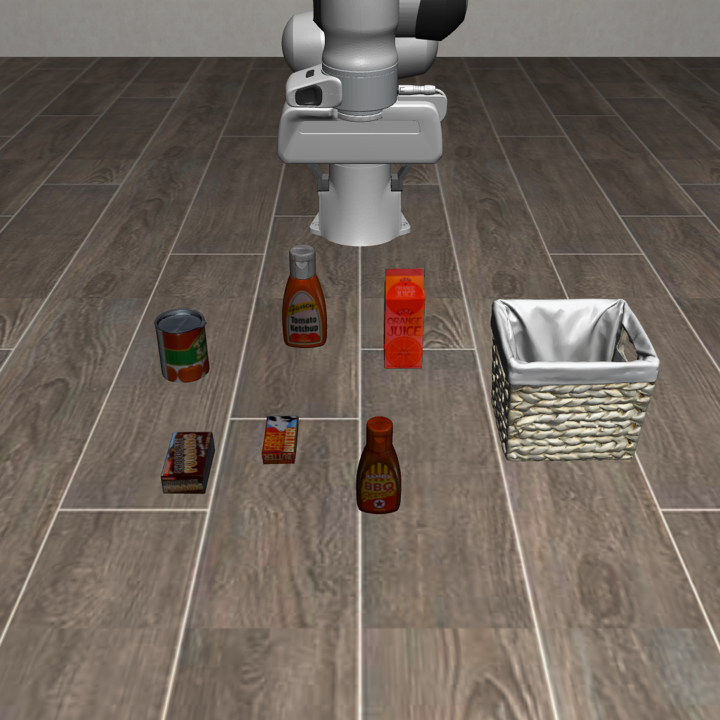
\includegraphics[width=0.47\textwidth]{figures/t6-butter-name-fails.png}\hfill
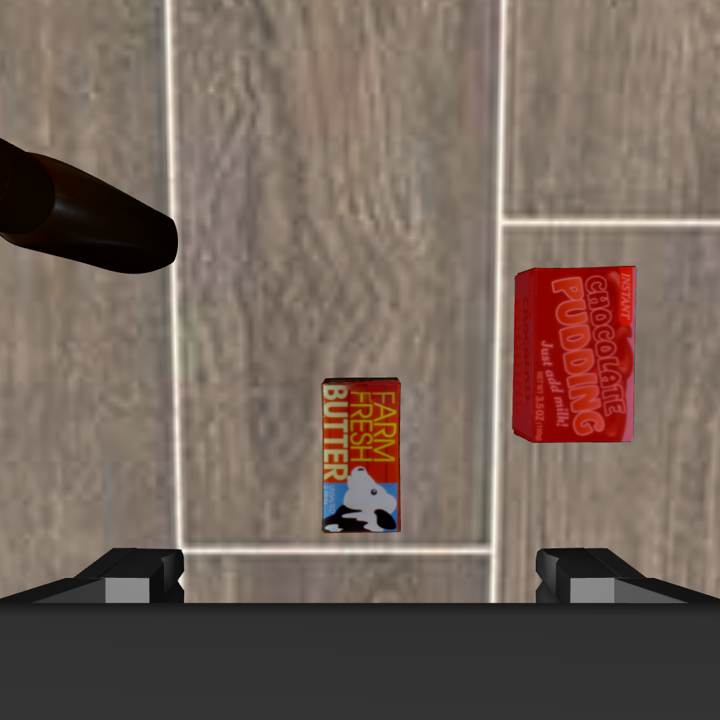
\includegraphics[width=0.47\textwidth]{figures/t6-shape-prompt-fails.png}
\caption[t6 为什么必须靠排除法]{\textbf{t6 为什么必须靠排除法定位。}\emph{左，agentview：}
提示词 \texttt{"yellow rectangular stick of butter"}（0.562）把掩膜打在了\textbf{橙汁盒}
上——而且返回的坐标与 \texttt{"orange juice carton"} 提示词（0.855）完全相同。真正的黄油
是桌面中偏左那个平躺的小盒子，标签清清楚楚，却完全没有被掩膜覆盖。\emph{右，腕部相机：}
一个基于形状的说法 \texttt{"flat rectangular block on the table"}（0.535）把掩膜打在了
\textbf{巧克力布丁盒}上，而 \textsc{farm fresh butter} 就摆在画面正中，未被掩膜。
\textbf{这次运行里没有任何一张叠加图显示黄油被正确分割，因为没有任何一种说法找到过它。}
真正奏效的定位完全没有用分割——用的是占据栅格扫描加一个“抬高薄板”判别式，它们产出的是
数字，不是叠加图。\textbf{这张缺席的图本身就是结论。}
来源：\texttt{exam1\_t6\_s0/segments/}，记录 \texttt{segment\_00\_09} 与
\texttt{segment\_01\_00}。}
\end{figure}


\begin{caution}[title={这个项目不得不纠正自己的一个说法}]
它在内部被写成了“历史上 0/11”。这是假的：这一格在沙箱存在\emph{之前}被解开过 6/7 次，
其中四次读了那一格的答案文件。准确的说法是\textbf{“净室时代 0/11”}——而这个说法更强。
\end{caution}

\section{t5：仪器是对的，规划器把它否决了}

装上仪器后 t5 只从 0/3 动到 1/3。两次失败按一套在扫描产出任何数字\emph{之前}就固定下来
的流程做了裁决，而答案不是设计所预期的。

从解开的那次运行确立的事实：目标是一个带红绿标签的银色\textbf{罐}；桌上另一处那个棕色
\textbf{瓶}上写着 “TANGY BBQ SAUCE”。两次失败都抓了那个瓶子——而且是在读图者已经正确地
把它认成 BBQ 之后——依据的是下面这条推断，引自智能体自己的审计：

\begin{evidence}[title={那条失败的推断}]
\small\itshape
“既然环境保证有一个可抓取的 \textrm{\texttt{tomato\_sauce\_1}}，而桌上恰好只有一个瓶子，
那就把这个立着的瓶子当作番茄酱。”
\end{evidence}

\noindent
番茄酱是一个\textbf{罐}。“唯一的瓶子”按构造就是那个干扰物。仪器工作正常；建立在它之上的
推断没有。

\begin{figure}[htbp]
\centering
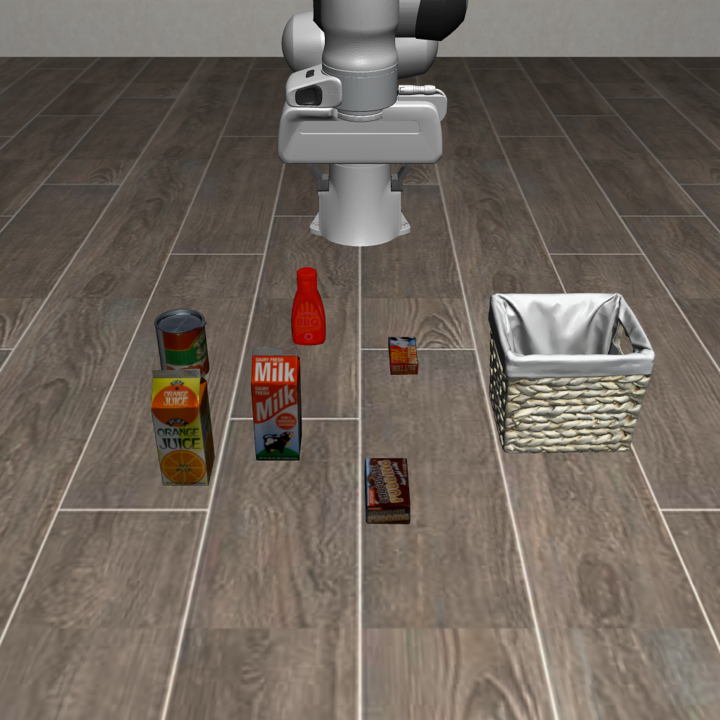
\includegraphics[width=0.47\textwidth]{figures/t5-collapse-bbq.png}\hfill
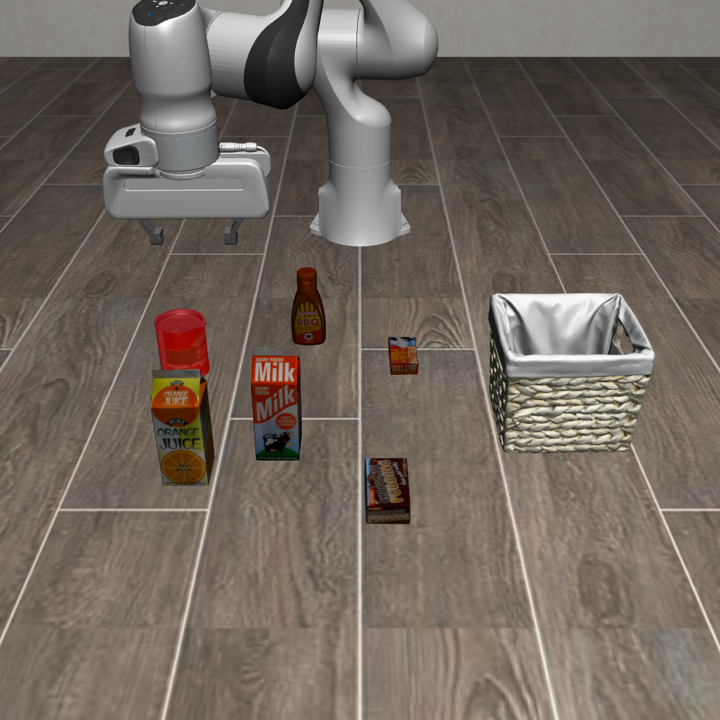
\includegraphics[width=0.47\textwidth]{figures/t5-target-can.png}
\caption[t5 的身份陷阱]{\textbf{t5 的身份陷阱，两张分割叠加图。}\emph{左：}提示词
\texttt{"bbq sauce bottle"} 得分 0.930，掩膜落在 $[-0.19,-0.074]$ 那个立着的瓶子上。
另外三个互斥的提示词——\texttt{"small red tomato sauce bottle"}（0.859）、
\texttt{"small red bottle"}（0.852）、\texttt{"brown sauce bottle"}（0.898）——返回
\emph{完全相同}的世界坐标。四个互不相容的名词，一个物体：这就是数据总线会报告、而任何
单个分数都看不出来的\textbf{塌缩}。\emph{右：}把名词从\emph{瓶}换成\emph{罐}，才找到真正
的目标——\texttt{"tomato sauce can"}（0.785），位于 $[-0.099,-0.237]$，橙汁盒后面那个
金属罐。
\textbf{读图提醒：}那层红色\emph{是掩膜}，不是物体本身的颜色。BBQ 瓶其实是棕色的——它在
右图未被掩膜时就是棕色；一旦被掩膜就显得发红，而这恰恰就是这一格所利用的那种混淆。
来源：\texttt{exam\_t5\_s0\_solved/segments/}，记录 \texttt{segment\_00\_02} 与
\texttt{segment\_02\_01}。}
\end{figure}


% ==========================================================================
\chapter{问题：已关闭与仍开放}

\section{门的引用够不到归档的尝试}

第一版尝试轮转把证据改名进一个归档目录，而引用解析器不读那里。于是在第一次真实的驻场
会话里，最关键的反驳证据\emph{无法被引用}，回放也把归档的回合报成记录缺口。这在批准这个
捷径时就被接受为技术债；引用语法需要一个可选的“尝试”段。\textbf{仍然开放}，而且它后来
还咬了挖掘那一侧：一条提案从挖掘器唯一能看到的那次尝试里做了过度概括。

\section{某个臂执行不了的知识}

条目可以预设工具。一个盲臂带着依赖视觉的条目，读到的是它无法照做的指令——这在结构化
“依赖”字段被定义时就预测过，随后被观察到：受影响那一格的两次盲态运行都读了它全部五条
条目，而仪器调用为零。补救办法是按运行的真实工具面过滤索引。这次暴露以“已观察”记录；
它的\emph{影响}仍未量化，因为转录还没有被读过。

\section{一天之内关闭：一条过了门的条目变成了借口}
\label{sec:5f}

这是本项目产出的最尖锐的否定结果，而且它针对的是\textbf{自己的机制}，不是模型的。

一条环境级条目——每一格都会读到——正确地记录了终止标志不是神谕，并要求在宣告成功前做至少
两项独立的物理检查。但它的收尾一句写着：\emph{如果物体已确认在篮子里、原位已空、而终止
仍未触发，就把任务视为完成。}

在仪器臂里，六次失败全都读了它，其中三次明确引用了它。而在其中两次里，智能体放进去的是
\textbf{错的物体}；检查器保持沉默是对的。这条条目递给一次“拿错东西”的运行一个现成的、
听起来很诚实的理由去停止寻找，而智能体接过它，写下了自信的审计——其中一次还填了“成功”
的状态。

\begin{caution}[title={为什么任何一项门检查都抓不到它}]
这条条目是\emph{真的}。它的引用能解析，数字能追溯，它自己的反证据块还诚实地声明了一个
它的配方失效的案例。它是被\textbf{正确地}准入的。缺陷在于：它的停止条件挂在“标志没有
触发”这个\emph{现象}上，而不区分\emph{为什么}没触发，于是在检查器错的时候和检查器对的
时候，它一视同仁地触发。这是\textbf{一条准许放弃的成长型知识}。
\end{caution}

\begin{resolved}[title={当天修复，而且是通过产生它的那道门}]
负责人批准了一批修订，堵住这个洞而不是删掉条目。该条款现在写的是：检查通过而标志沉默，
这是智能体自身验证与环境评分权威之间的一个\textbf{矛盾}——而标志才是权威。它还写明了
为什么“在场检查”解决不了这件事：\emph{把错的物体放进篮子，能通过其中每一项检查，而检查
器沉默得完全正确。}在停止之前，必须验证篮子里那个物体的\textbf{身份}：装配了视觉通道就
读它的标签，否则把实测几何与目标的特征签名做匹配。只有在已验证的\textbf{目标}确实在里面、
而标志仍然沉默时，才可以考虑检查器不稳定，并且必须把这个矛盾明确写进审计、以一个诚实的
状态收尾——\textbf{绝不能是一个不加限定的“成功”}。

同批还改了两条：这一格的“检查器不稳定”主张被下调为“一次未经确认的重复”，因为它三次支持
性证据里有两次现在已由“拿错物体”解释；另外新增一条记录目标是罐而不是瓶，使“唯一的瓶子”
那条推断\textbf{按构造即为无效}。
\end{resolved}

\noindent
这个循环本身值得作为一项结果来命名：\textbf{一天之内被设计、被诊断、被修复}，而且是由
准入了这个缺陷的同一条流水线完成的——从运行记录中观察、由人裁决、经门修订，每一步都附着
运行引用。

\section{仍然开放}

四条中间件已具名但未实现：按组件的 token 记账、带影子模式的硬门、参数级 provenance、
以及考试运行的上下文压缩。感知栈有一个已知缺口，多候选歧义会被静默塌缩。跨相机掩膜融合
尚未实现。还有一个测试断言了一条设计\textbf{刻意不提供}的顺序性质——日志按完成顺序排列、
按调用 id 连接，恰恰是因为位置不可靠——所以该修的是测试。

% ==========================================================================
\chapter{定位}

审稿人的第一个问题会是：为什么不直接用现成的智能体框架。因为桌面型智能体框架编码了四条
在具身场景下会破掉的假设。

\keyrule{动作可逆且便宜}，所以它们优化吞吐——并行、投机执行、子智能体扇出。具身要求的是
\textbf{先证据后承诺}：推进/只读划分、新鲜度判定、动作后验证。

\keyrule{世界就是文本}，所以它们有虚拟文件系统。这里重数据在磁盘上、引用进上下文；文本
只是一次\emph{经由测量的投影}。

\keyrule{存在一个便宜的判定器}——“跑测试就行”。具身必须\emph{自己造}判定器，而且环境自己
的标志会撒谎，两个方向都会，本文已经展示了两次。

\keyrule{任务可以分解成互不相干的上下文。} 一个回合是一个连续的世界和一具身体。只有对已
落盘产物的只读感知可以扇出。

框架的图执行引擎是共用的底盘。这套框架长了两遍：一遍是\textbf{手工长的}，由具身约束乘以
项目自己的规矩长出来；一遍是\textbf{自己长的}，经由门生长，而且生长本身被测量。最近的
邻居被引用而不是被无视——一篇已发表的系统拥有驻场会话机制和逐原语轨迹引擎（其消融是该文
最大的效应），但没有测量自己的生长；另一篇是真机上的同类，但记忆是自由写入的；第三篇在
三个具名的地方领先，包括把“工具完成”“世界状态改变”“任务成功”当作三个不同的主张——这个
框架现在被引用在本项目自己的工具契约里。

% ==========================================================================
\chapter{复现}

每一条主张都可以在不安装智能体框架的情况下，从运行归档中重新算出来。成绩来自步骤轨迹；
包含只读调用在内的逐调用记录来自调用日志；每次运行的边界来自它的沙箱指纹。

\begin{evidence}[title={检查}]
\ttfamily\footnotesize
\# 这次运行消费过先验吗？（对每一个沙箱化的运行都应为空）\\
grep 'read\_text\_file' run.log | grep -E 'results\_.*\_pert|env\_calibration'\\[0.5em]
\# 只凭磁盘重建任意一次运行的证据\\
python -m rpent.replay \textless run\_dir\textgreater\\[0.5em]
\# 回归测试：不需要 API key，不需要 GPU——13 个测试\\
for t in deep\_agent resident vision\_tool tool\_docs prompt\_leveling sandbox \textbackslash\\
\hspace*{2.2em}databus shape gate practice replay locateanything; do \textbackslash\\
\hspace*{2.2em}python tests/harness/test\_\$t.py; done
\end{evidence}

\vspace{1em}
\begin{center}
\textit{本文中的数字，好不过 §\ref{sec:counting} 里那些约定。\\ 而那些约定之所以存在，是因为更早的数字
并不好。}
\end{center}

\end{document}
